\section{Resultados.}

\subsection{ID3.}

En los gráficos siguientes se muestran los 21 modelos diferentes que se construyeron combinando las diferentes variables para entrenar el modelo con el algoritmo ID3. En color verde están marcadas las variables utilizadas en cada modelo. En la primera de las dos filas inferiores se muestra el porcentaje de instancias del conjunto de entrenamiento clasificadas correctamente por el algoritmo.

En la segunda de las dos filas inferiores se muestra el porcentaje de target para los modelos potenciales seleccionados como candidatos para ser el clasificador referencia construido con el algoritmo ID3. Como puede apreciarse el modelo V0, con todas las variables introducidas, clasifica correctamente prácticamente todas las instancias del conjunto de entrenamiento pero presenta un gran sobreajuste sobre esos mismas instancias. Esto se refleja en los resultados sobre el conjunto de validación.

En este caso, el modelo de referencia sería el V3 o el V20.

\begin{figure}[H]
\begin{center}
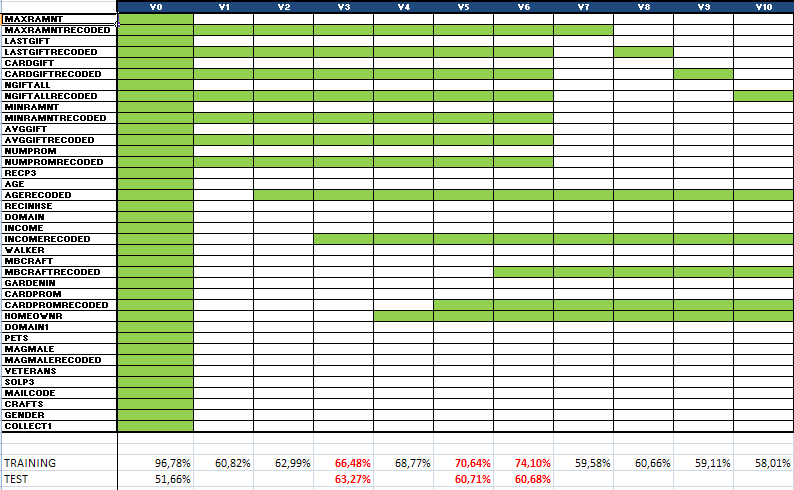
\includegraphics[width=0.9\textwidth]{img/id3-1}
\caption{Modelos construidos con el algoritmo ID3.}
\end{center}
\end{figure}

\begin{figure}[H]
\begin{center}
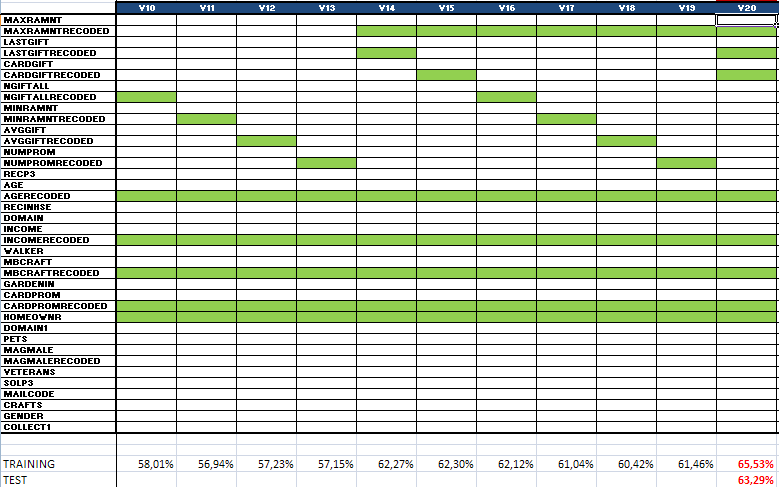
\includegraphics[width=0.9\textwidth]{img/id3-2}
\caption{Modelos construidos con el algoritmo ID3.}
\end{center}
\end{figure}

\subsection{J48.}

A continuación se muestra la información de los diferentes modelos construidos con el algoritmo J48. En este caso los modelos de referencia son el V5 y el V11. Aunque resulte extraño, no ha sido posible mejorar los resultados obtenidos con el algoritmo ID3.

\begin{figure}[H]
\begin{center}
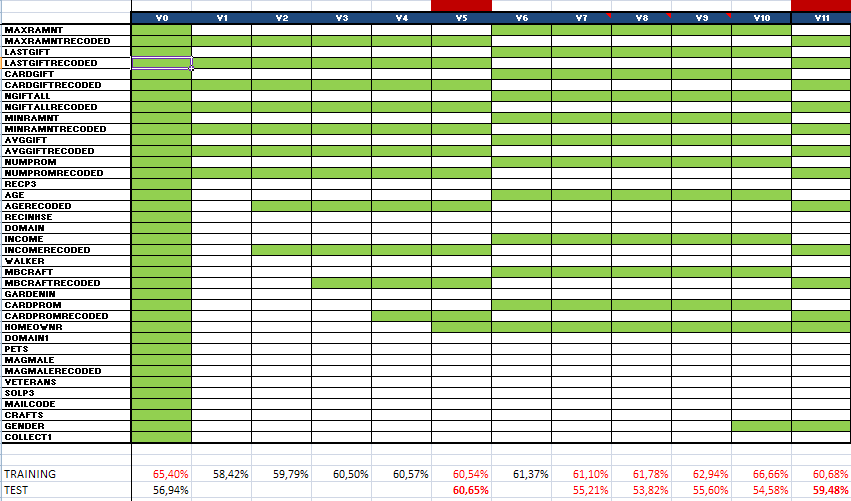
\includegraphics[width=0.9\textwidth]{img/j48-1}
\caption{Modelos construidos con el algoritmo J48.}
\end{center}
\end{figure}

Y esta es la tabla que muestra los diferentes parámetros probados previos al desarrollo de los modelos:

\begin{figure}[H]
\begin{center}
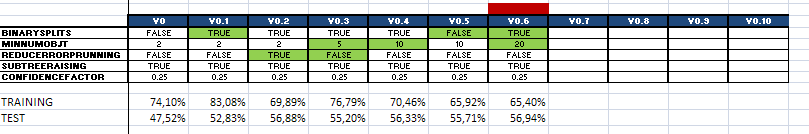
\includegraphics[width=0.9\textwidth]{img/j48-2}
\caption{Pruebas de los diferentes parámetros de configuración del algoritmo J48.}
\end{center}
\end{figure}

A continuación se muestra una captura de pantalla de la salida del algoritmo mostrada por la herramienta Weka:

\begin{figure}[H]
\begin{center}
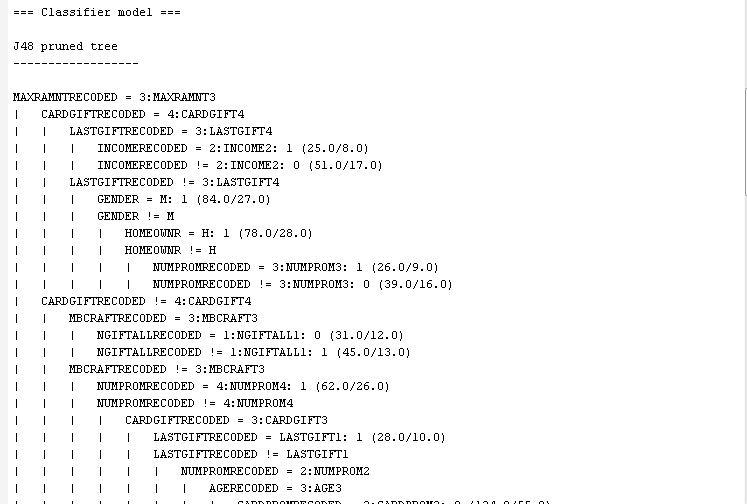
\includegraphics[width=0.9\textwidth]{img/j48-3}
\caption{Salida parcial de la herramienta WEKA del modelo construido con el algoritmo J48.}
\end{center}
\end{figure}

\subsection{M5P.}

La variable target es una variable discreta y no ha sido posible probar el algoritmo M5P.

\subsection{IB1.}

A continuación se muestra la información de los diferentes modelos construidos con el algoritmo IB1. En este caso no se ha seleccionado ningún modelo de referencia dado que todos los construidos tiene resultados muy por debajo de los obtenidos con los algoritmos anteriores.

\begin{figure}[H]
\begin{center}
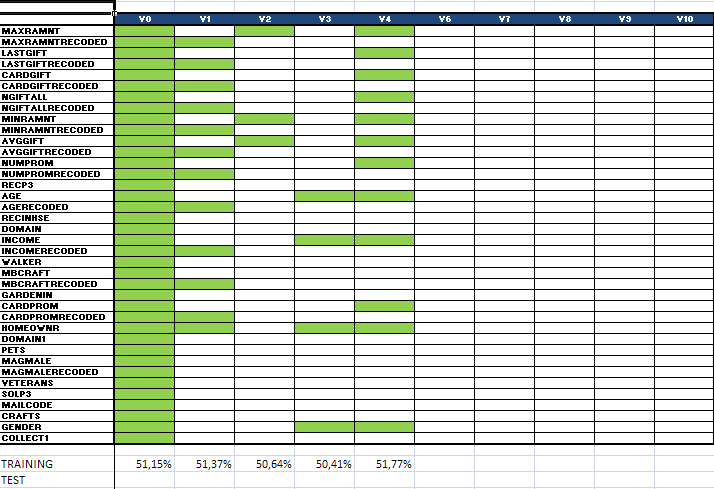
\includegraphics[width=0.9\textwidth]{img/ib1-1}
\caption{Modelos construidos con el algoritmo IB1.}
\end{center}
\end{figure}

\subsection{IBK.}

A continuación se muestra la información de los diferentes modelos construidos con el algoritmo IB1. En este caso no se ha seleccionado ningún modelo de referencia dado que todos los construidos tiene resultados muy por debajo de los obtenidos con los algoritmos anteriores.

\begin{figure}[H]
\begin{center}
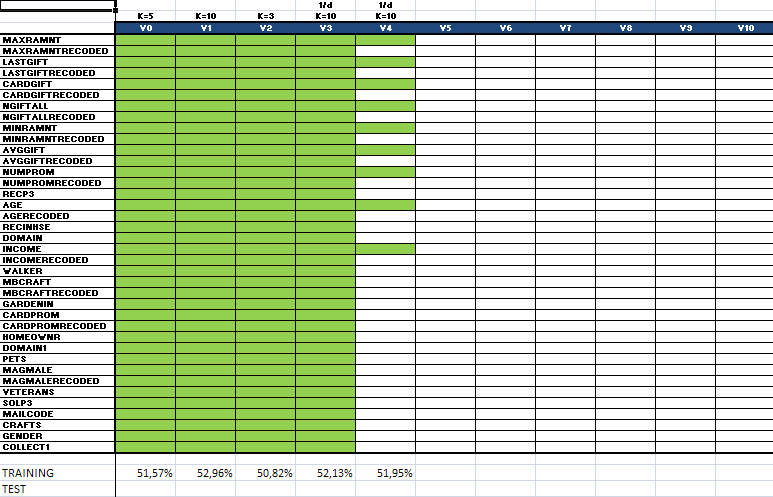
\includegraphics[width=0.9\textwidth]{img/ibk-2}
\caption{Modelos construidos con el algoritmo IBK.}
\end{center}
\end{figure}

Como puede observarse los mejores resultados se obtuvieron configurando el algoritmo con 10 vecinos y pesando por el inverso de la distancia.

A continuación se muestra una captura de pantalla de la salida del algoritmo mostrada por la herramienta Weka:

\begin{figure}[H]
\begin{center}
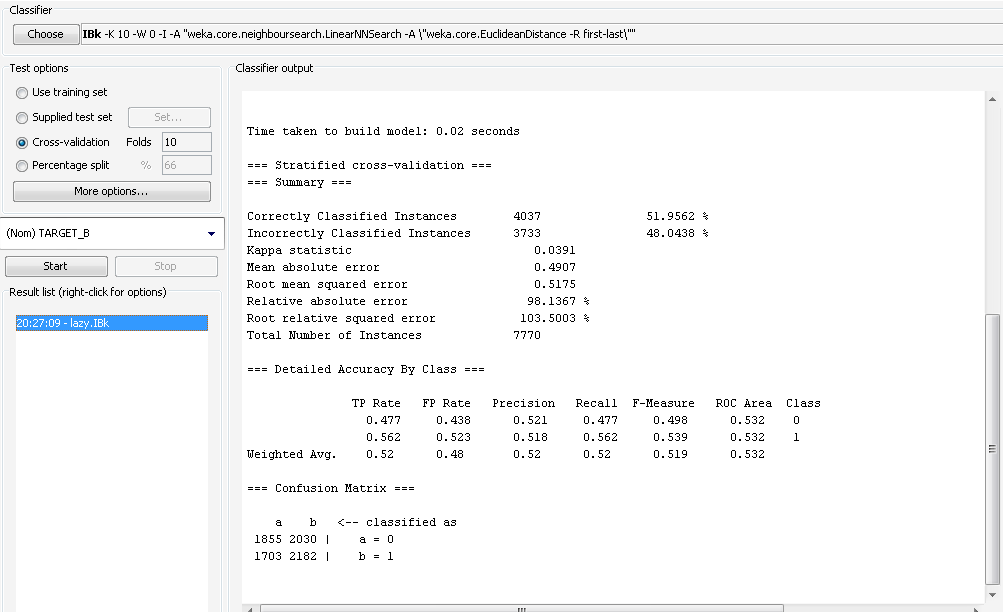
\includegraphics[width=0.9\textwidth]{img/ibk-1}
\caption{Salida parcial de la herramienta WEKA del modelo construido con el algoritmo IBk.}
\end{center}
\end{figure}

\subsection{Naive Bayes.}

A continuación se muestra la información de los diferentes modelos construidos con el algoritmo Naive Bayes. En este caso se ha seleccionado el modelo V2 como modelo de referencia aunque su <<performance>> es inferior a la obtenida con los algoritmos ID3 y J48.

\begin{figure}[H]
\begin{center}
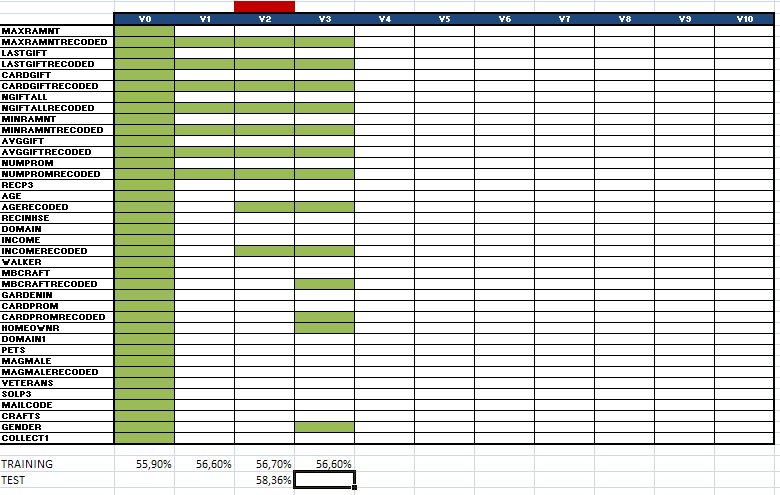
\includegraphics[width=0.9\textwidth]{img/nb-1}
\caption{Modelos construidos con el algoritmo Naive Bayes.}
\end{center}
\end{figure}

\subsection{TAN.}

A continuación se muestra la información de los diferentes modelos construidos con el algoritmo TAN. No se observa mejora respecto a los construidos con el algoritmo Naive Bayes y no se ha seleccionado ningún modelo de referencia.

\begin{figure}[H]
\begin{center}
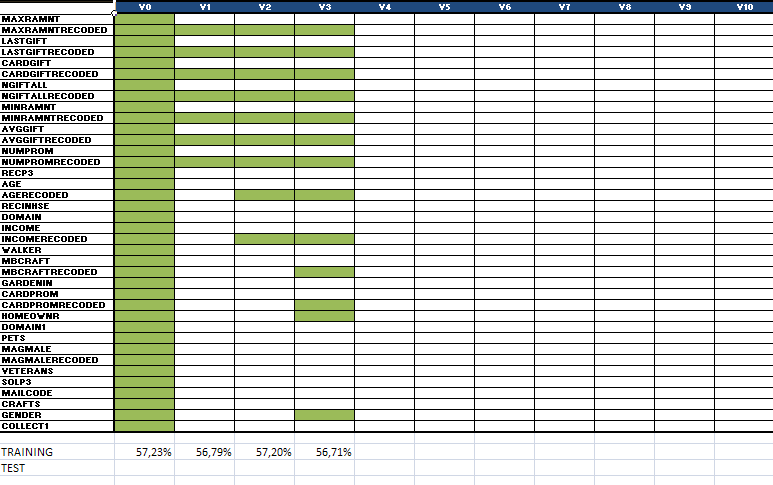
\includegraphics[width=0.9\textwidth]{img/tan-1}
\caption{Modelos construidos con el algoritmo TAN.}
\end{center}
\end{figure}

\subsection{Logistic.}

A continuación se muestra la información de los diferentes modelos construidos con el algoritmo Logistic. No se observa mejora respecto a los construidos con los algoritmos ID3 y J48 y no se ha seleccionado ningún modelo de referencia.

\begin{figure}[H]
\begin{center}
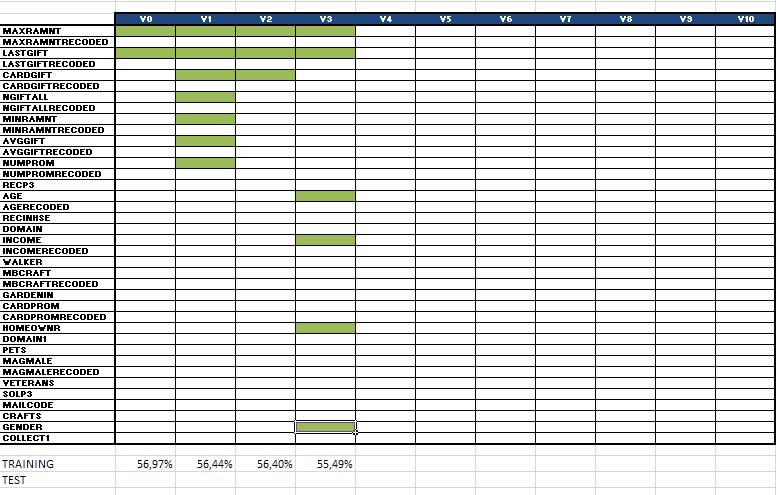
\includegraphics[width=0.9\textwidth]{img/logistic-2}
\caption{Modelos construidos con el algoritmo LOGISTIC.}
\end{center}
\end{figure}

Y una captura de pantalla de la herramienta WEKA mostrando las Betas asociadas a cada una de las variables del modelo V4:

\begin{figure}[H]
\begin{center}
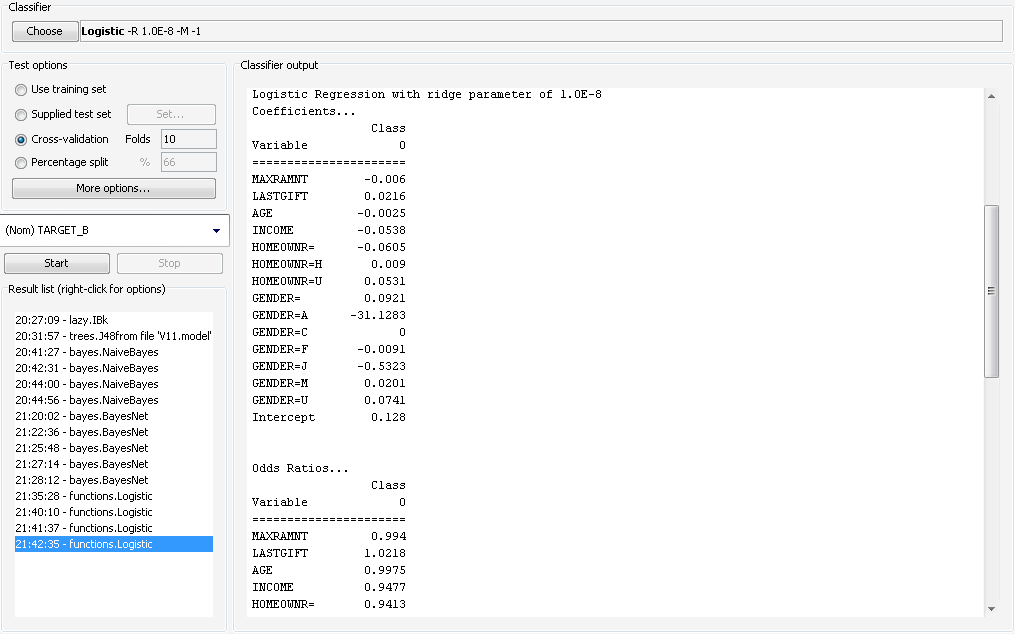
\includegraphics[width=0.9\textwidth]{img/logistic-1}
\caption{Salida parcial de la herramienta WEKA del modelo construido con el algoritmo LOGISTIC.}
\end{center}
\end{figure}

\subsection{JRIP.}

A continuación se muestra la información de los diferentes modelos construidos con el algoritmo JRIP:

\begin{figure}[H]
\begin{center}
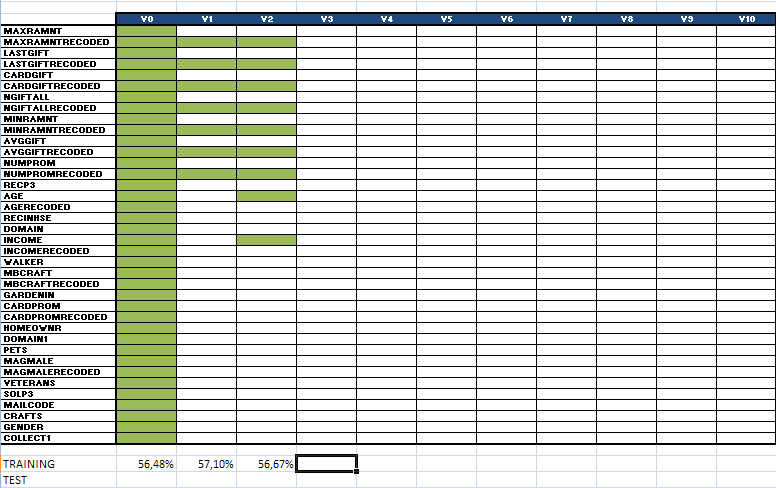
\includegraphics[width=0.9\textwidth]{img/jrip-2}
\caption{Modelos construidos con el algoritmo JRIP.}
\end{center}
\end{figure}

Y una captura de pantalla de la herramienta WEKA mostrando las reglas inducidas por el algoritmo:

\begin{figure}[H]
\begin{center}
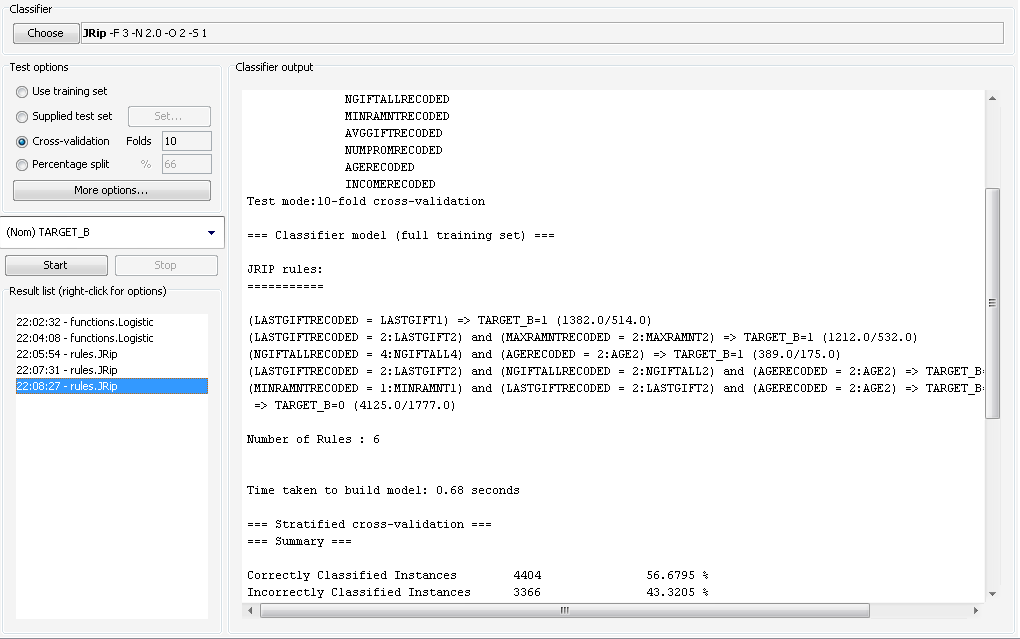
\includegraphics[width=0.9\textwidth]{img/jrip-1}
\caption{Salida parcial de la herramienta WEKA del modelo construido con el algoritmo JRIP.}
\end{center}
\end{figure}